\documentclass{beamer}

\usepackage{paratype}
\setbeamerfont{frametitle}{family=\bf}
\usepackage{listings}
\usepackage{pdfpages}

\lstset{
  language=C,
  keepspaces=true,
  moredelim=**[is][\color{red}]{@}{@},
}

% Beamer theme settings
\usecolortheme{seagull}
\usenavigationsymbolstemplate{} % no navigation buttons

\usepackage[utf8]{inputenc}

\title{OpenCL day 1: GPU hardware and the programming model}

\author{Cosmin Oancea and Troels Henriksen}

\date{January 28, 2019}

\begin{document}

\frame{\titlepage}

\section{Introduction and Course Contents}

\begin{frame}
  \tableofcontents[currentsection]
\end{frame}

\section{Hardware Trends}

\begin{frame}
	\tableofcontents[currentsection]
\end{frame}


\begin{frame}
  \frametitle{The first computers were not this}

  \begin{center}
    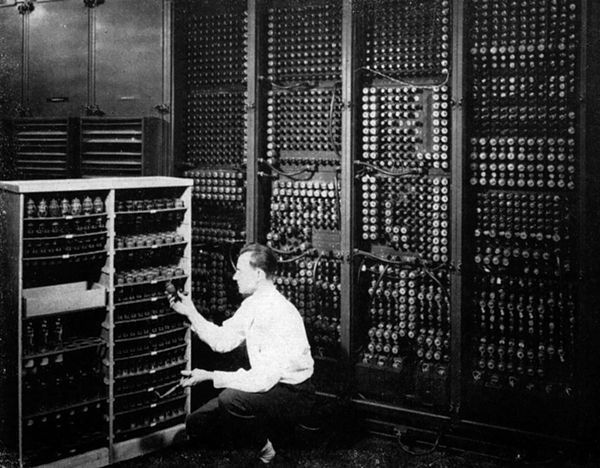
\includegraphics[width=\textwidth]{img/eniac.jpg}
  \end{center}

\end{frame}

\begin{frame}
  \frametitle{But this}

  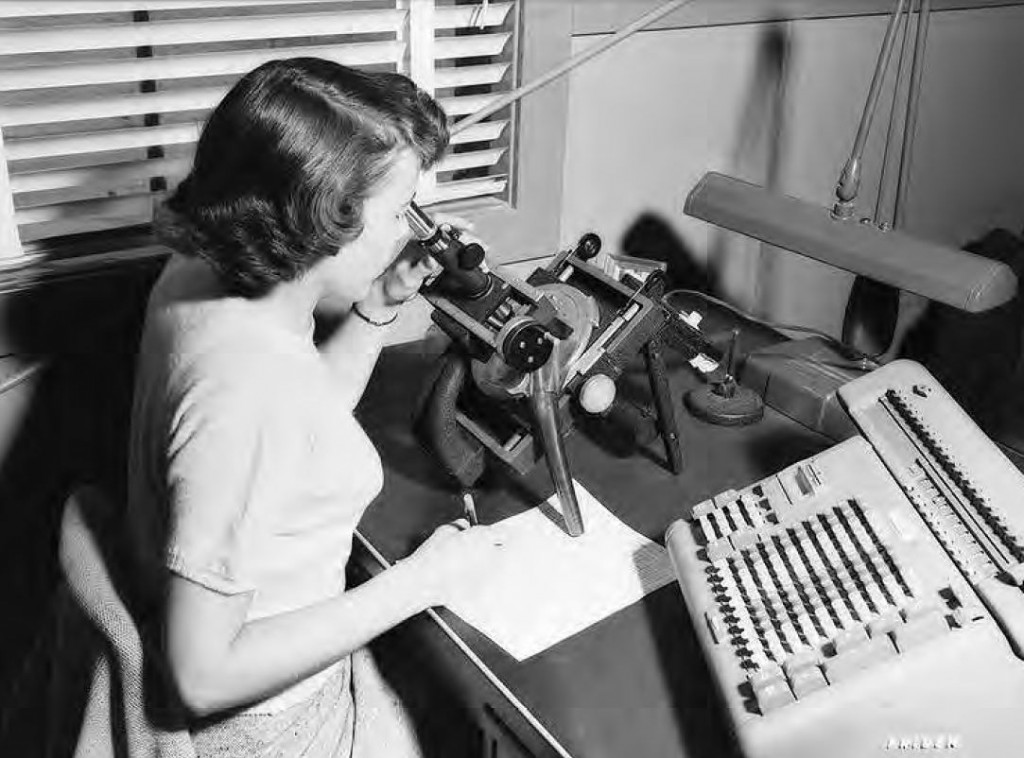
\includegraphics[width=\textwidth]{img/human-computer.jpg}
\end{frame}

\begin{frame}
  \frametitle{And if you had a larger problem}

  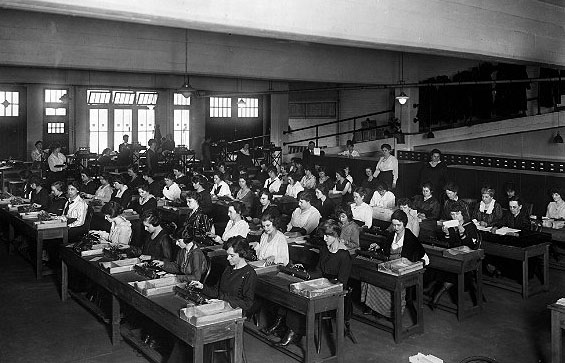
\includegraphics[width=\textwidth]{img/human-computers.jpg}
\end{frame}

\begin{frame}
  \frametitle{But then they started looking like this}

  \begin{center}
    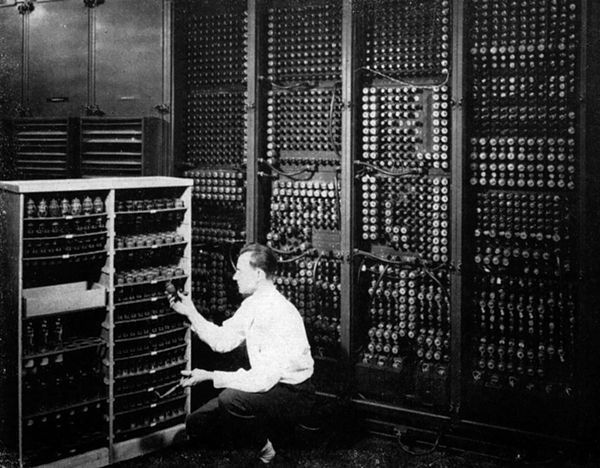
\includegraphics[width=\textwidth]{img/eniac.jpg}
  \end{center}
\end{frame}

\begin{frame}
  \frametitle{Then this}
  \begin{center}
    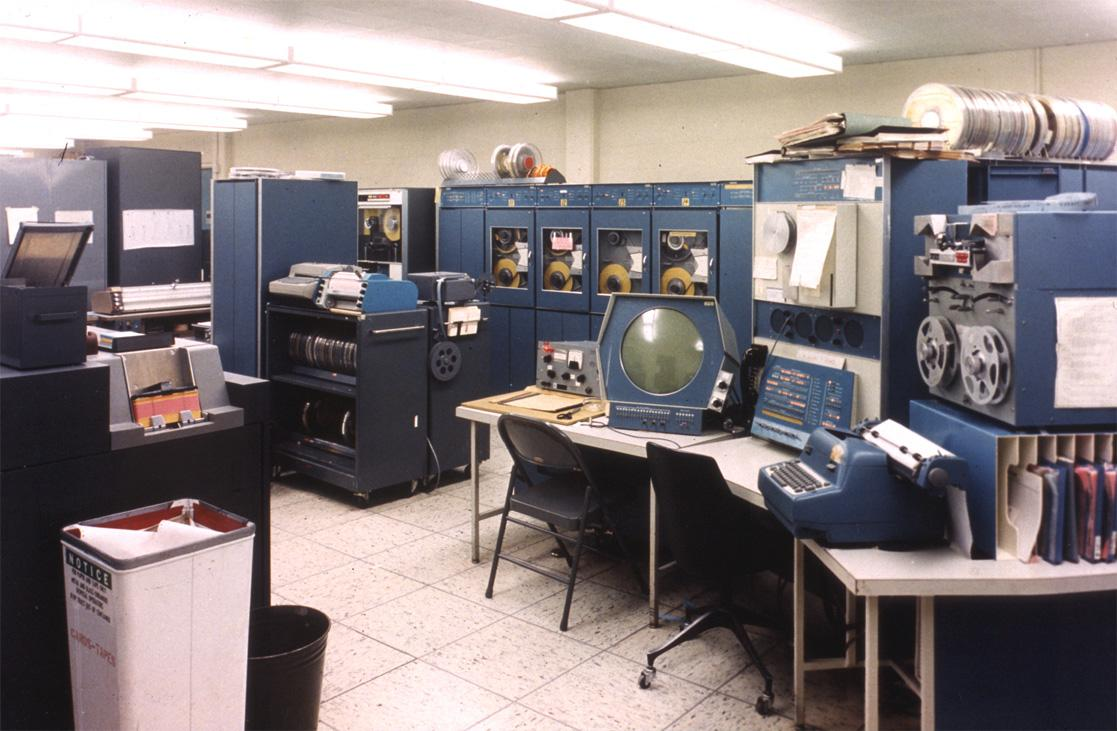
\includegraphics[width=\textwidth]{img/pdp1.jpg}
  \end{center}
\end{frame}

\begin{frame}
  \frametitle{Then this}
  \begin{center}
    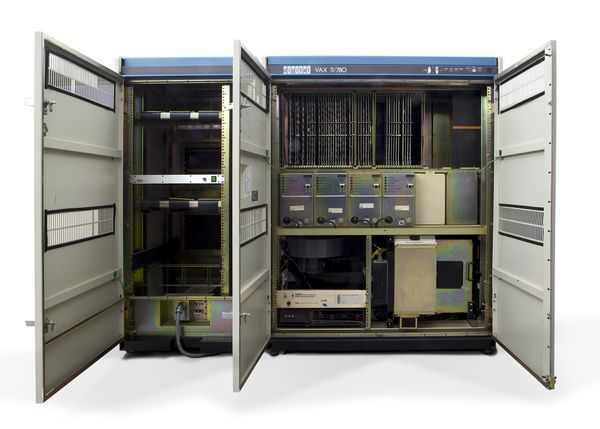
\includegraphics[width=\textwidth]{img/vax.jpg}
  \end{center}
\end{frame}

\begin{frame}
  \frametitle{Then this}
  \begin{center}
    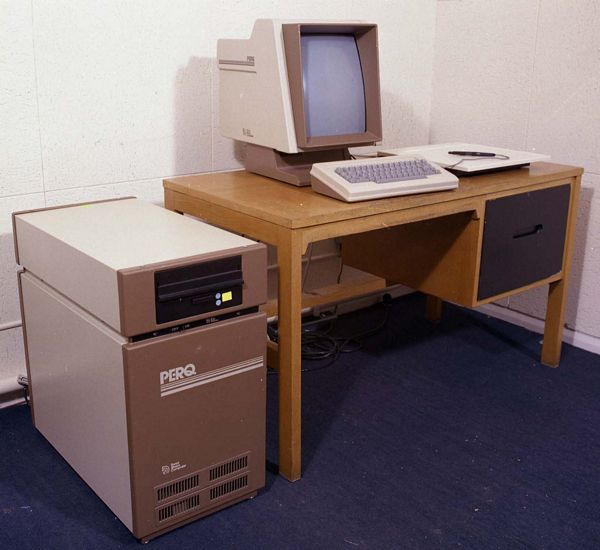
\includegraphics[width=\textwidth]{img/early-workstation.jpg}
  \end{center}
\end{frame}

\begin{frame}
  \frametitle{Then this}
  \begin{center}
    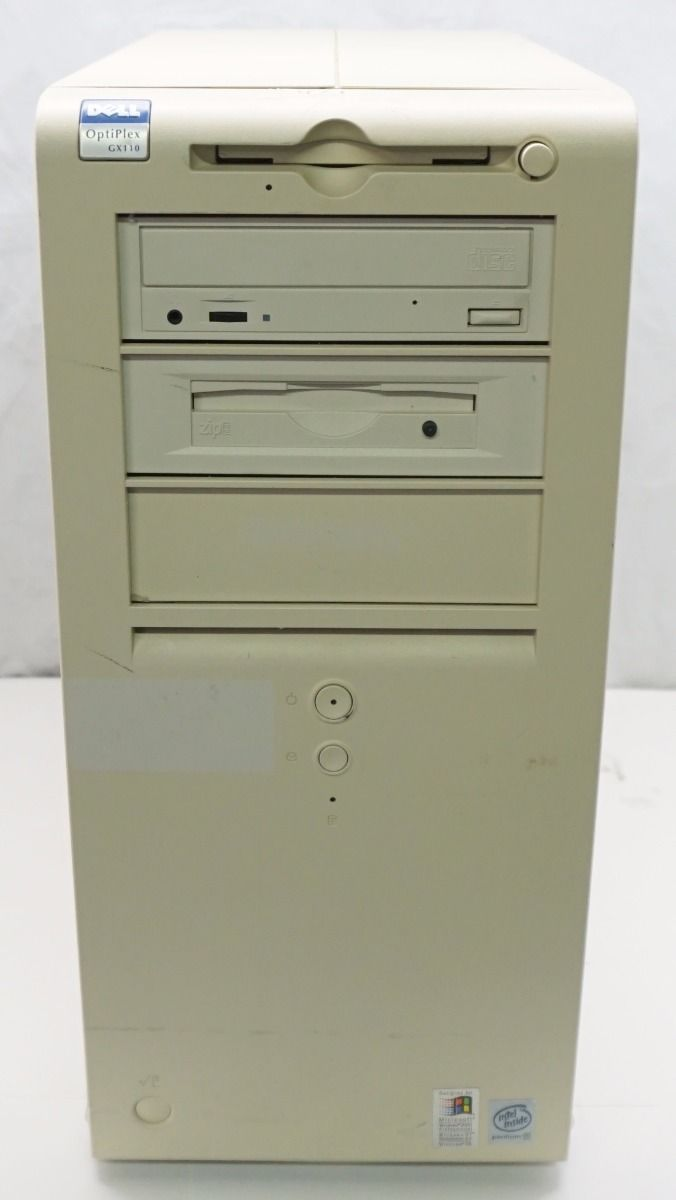
\includegraphics[width=\textwidth]{img/dell.jpg}
  \end{center}
\end{frame}

\begin{frame}
  \frametitle{Then this}
  \begin{center}
    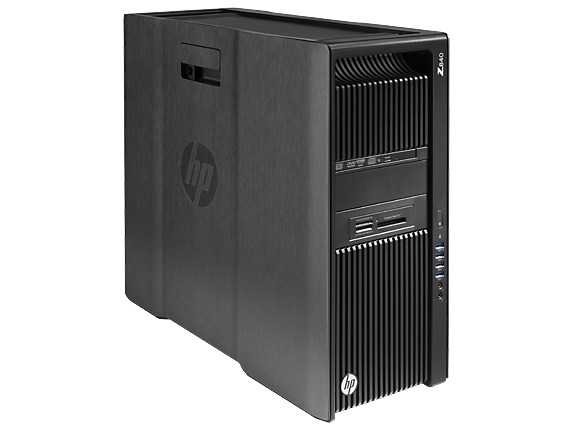
\includegraphics[width=\textwidth]{img/hp.jpg}
  \end{center}
\end{frame}

\begin{frame}
  \frametitle{Then, from around 2005}
  \begin{center}
    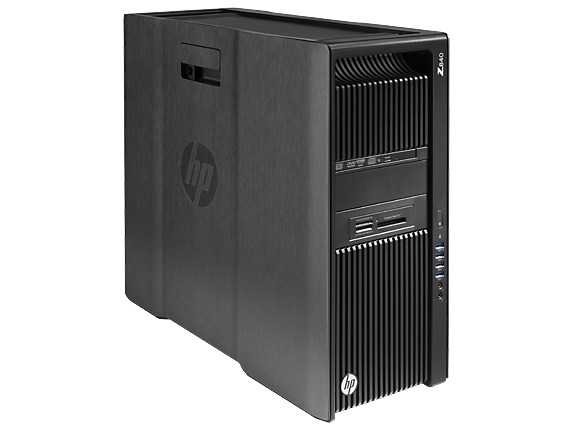
\includegraphics[width=0.5\textwidth]{img/hp.jpg}
    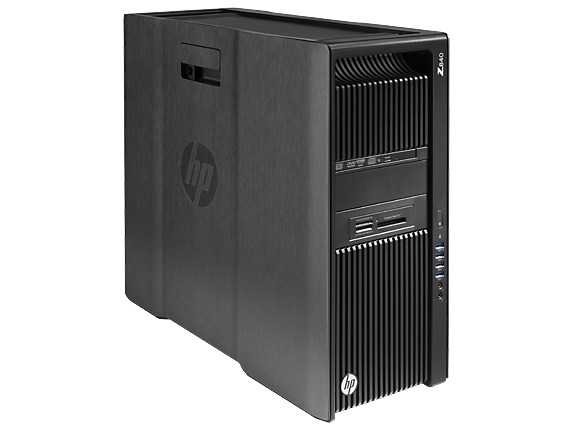
\includegraphics[width=0.5\textwidth]{img/hp.jpg}
  \end{center}
\end{frame}

\begin{frame}
  \frametitle{Then, from around 2005}
  \begin{center}
    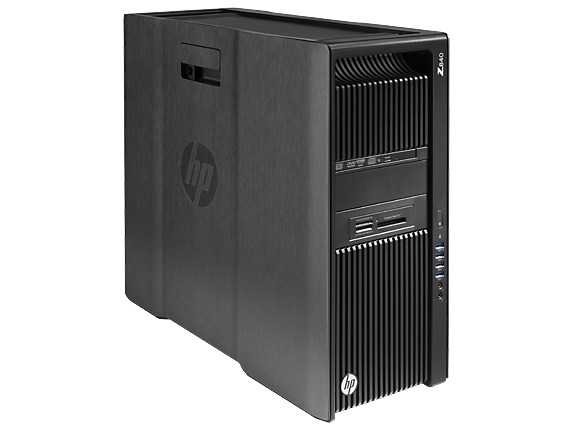
\includegraphics[width=0.3\textwidth]{img/hp.jpg}
    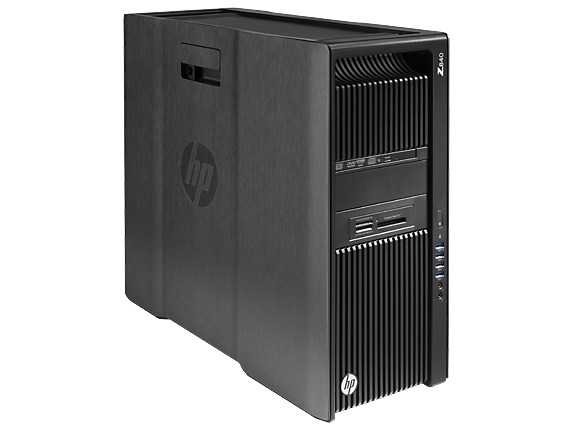
\includegraphics[width=0.3\textwidth]{img/hp.jpg}
    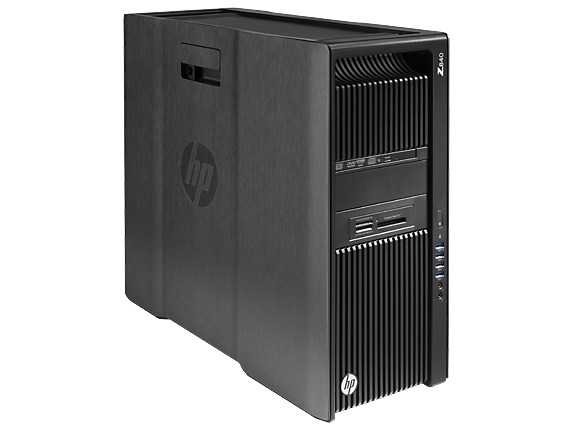
\includegraphics[width=0.3\textwidth]{img/hp.jpg}
  \end{center}

\end{frame}

\begin{frame}
  \frametitle{Then, from around 2005}
  \begin{center}
    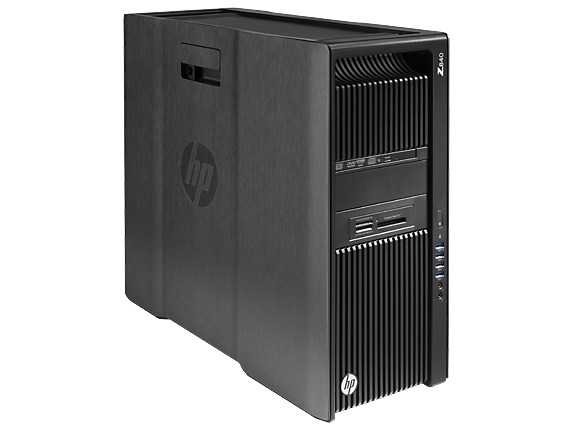
\includegraphics[width=0.3\textwidth]{img/hp.jpg}
    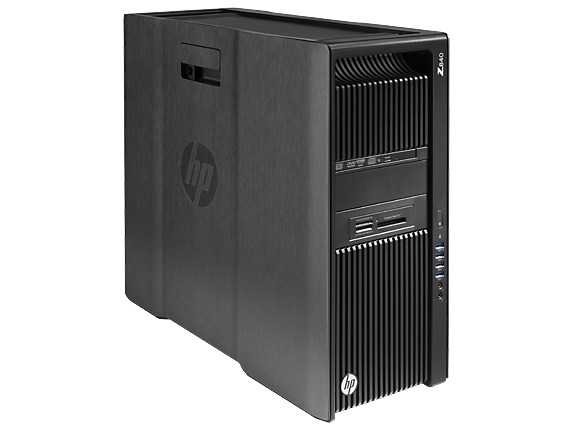
\includegraphics[width=0.3\textwidth]{img/hp.jpg}
    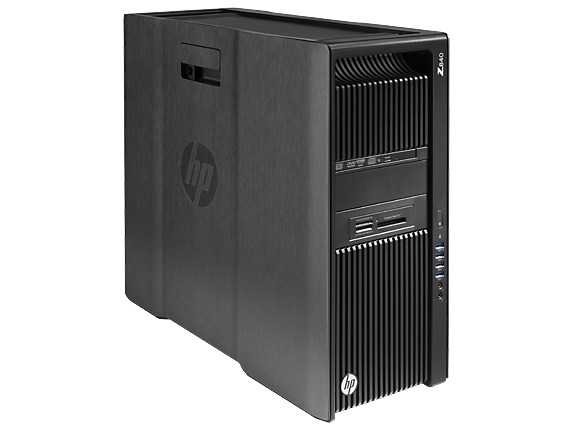
\includegraphics[width=0.3\textwidth]{img/hp.jpg}

    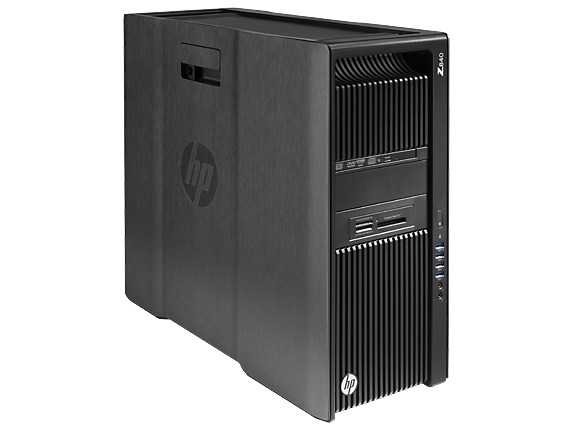
\includegraphics[width=0.3\textwidth]{img/hp.jpg}
    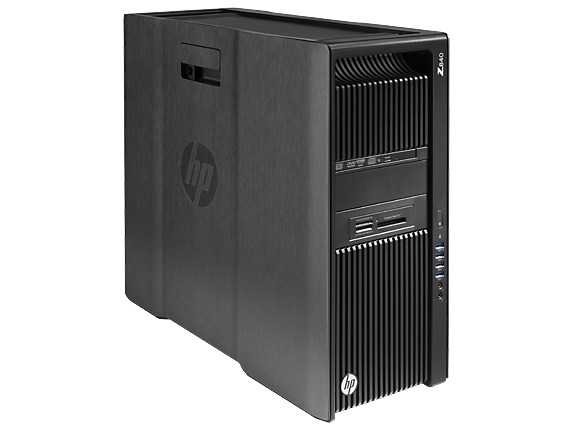
\includegraphics[width=0.3\textwidth]{img/hp.jpg}
    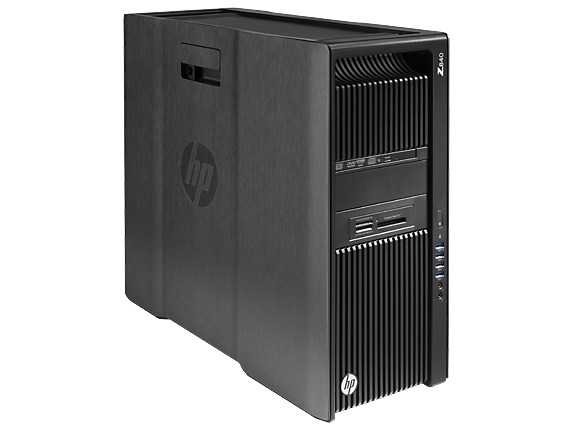
\includegraphics[width=0.3\textwidth]{img/hp.jpg}
  \end{center}

  Improvements in \textit{sequential performance} stalled, although
  computers still got smaller and faster.
\end{frame}

\begin{frame}
  \frametitle{What Changed?}

  \begin{itemize}
  \item \textit{Power complexity} $P_{dynamic} \sim Freq^3$,
    preventing us from increasing processor frequency.
  \item \textit{Memory wall}, ever-increasing performance gap between
    processor \& memory (which means that \textit{memory} becomes
    bottleneck, not processor speed).
  \end {itemize}
\end{frame}

\begin{frame}
  \frametitle{CPU progress}

  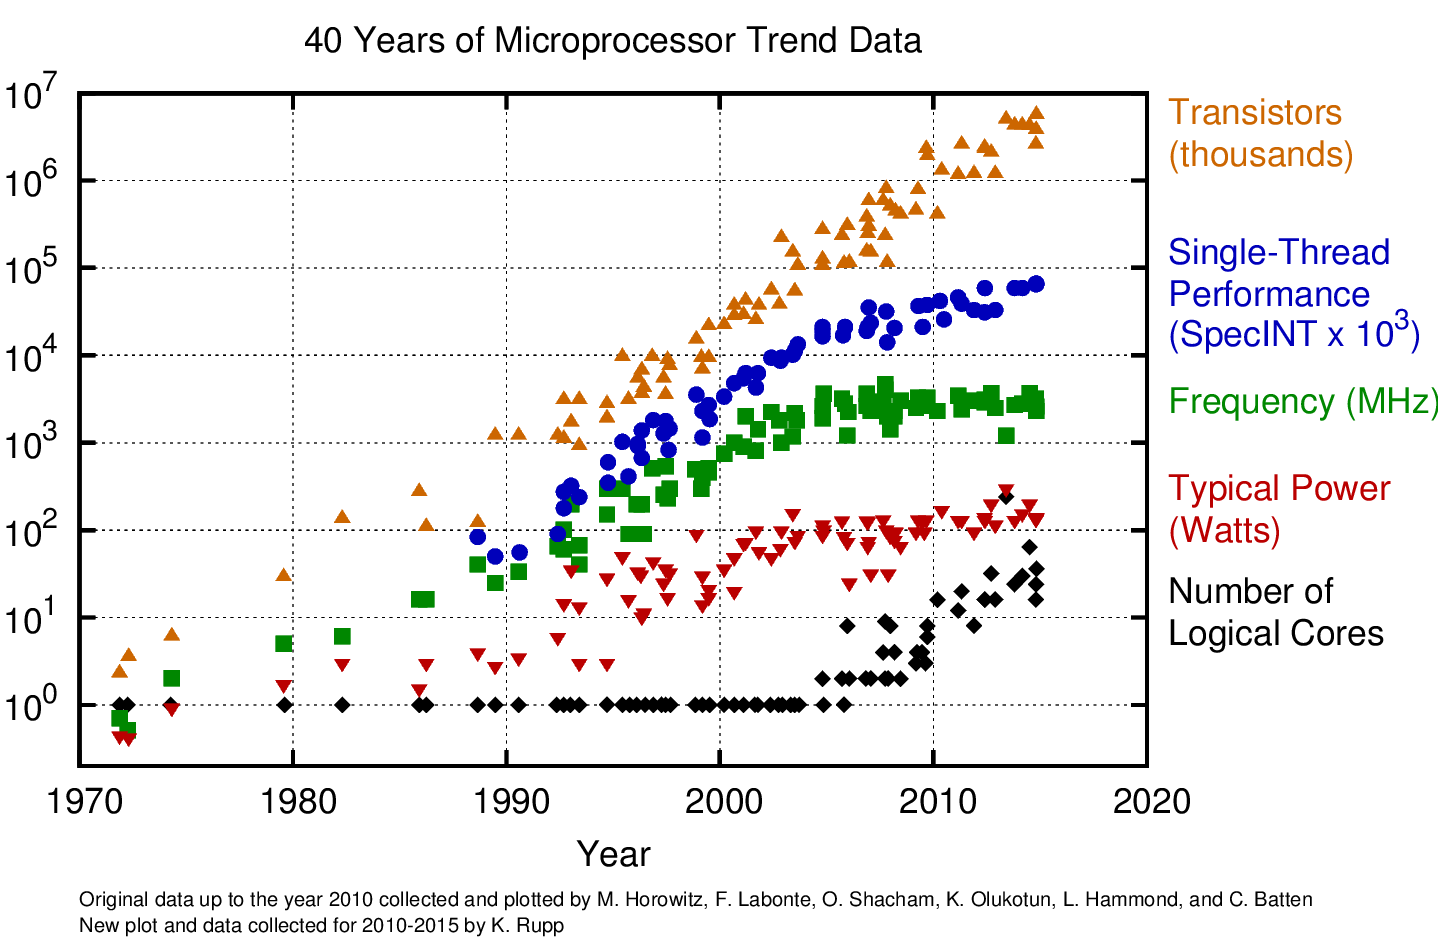
\includegraphics[width=\textwidth]{img/40-years-processor-trend.png}

Addressed with \textit{more cores}.

\end{frame}

\begin{frame}
  \frametitle{The Memory Wall}

\begin{center}
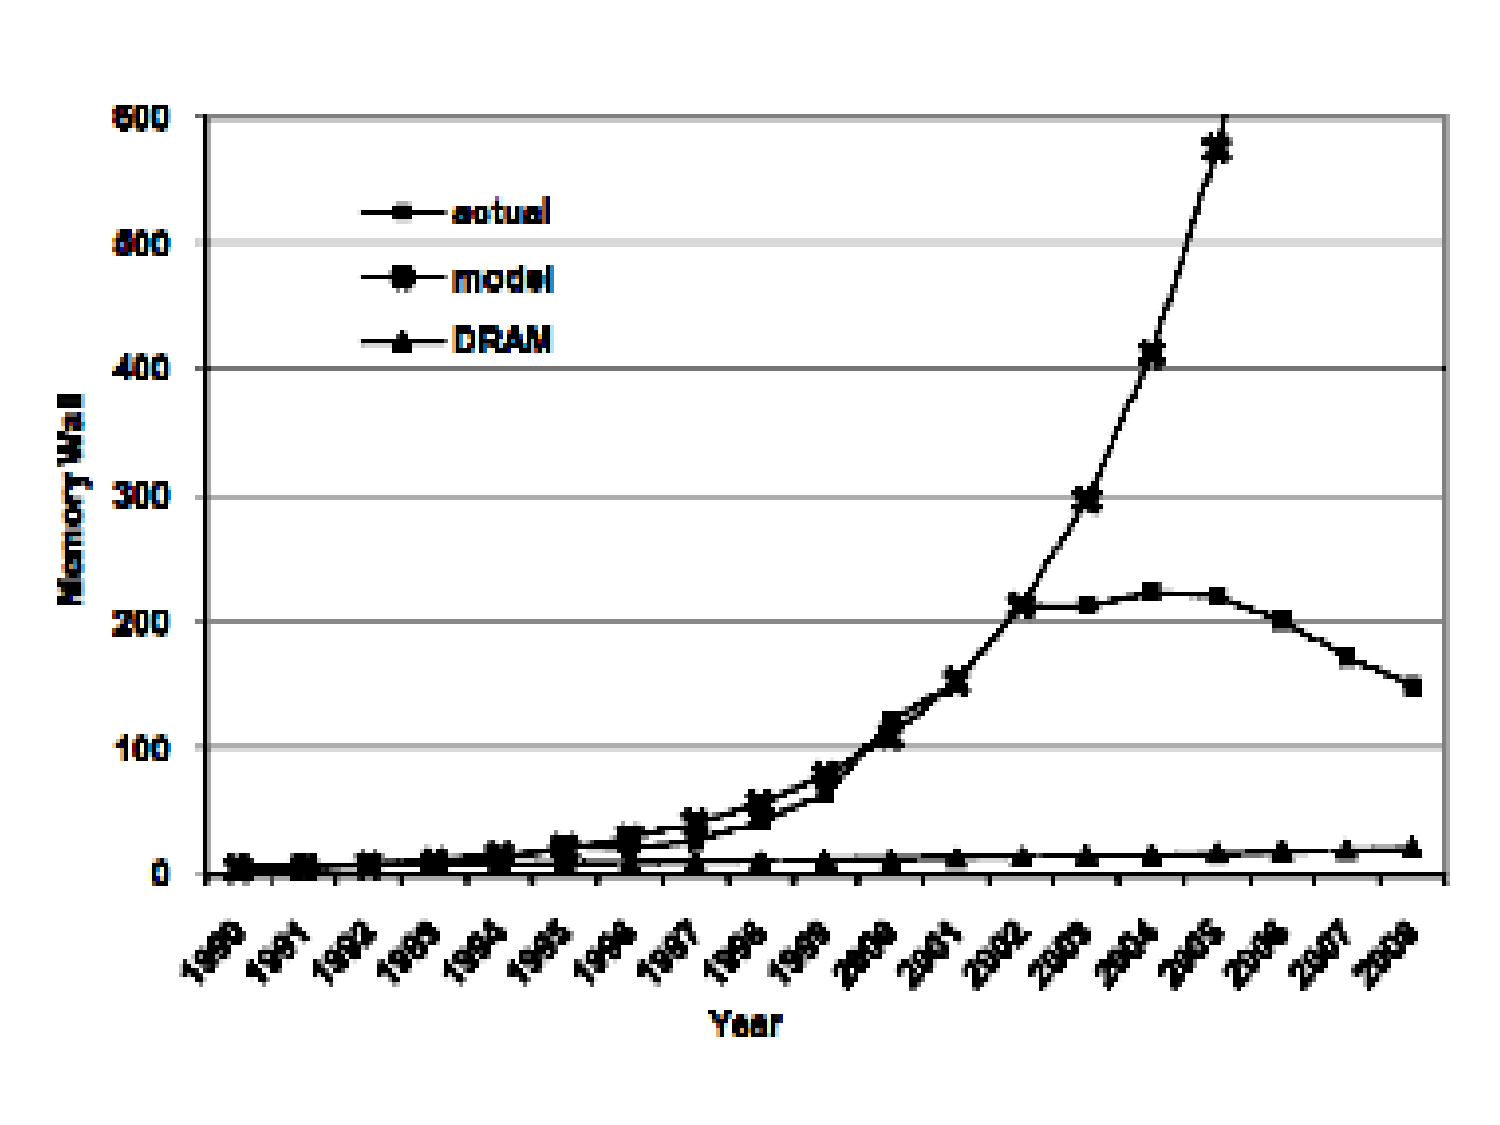
\includegraphics[width=50ex]{img/memwall}

  Memory Wall = $\text{processor cycles} / \text{memory cycles}$
\end{center}

Addressed with caches (not scalable) and \textit{latency hiding}.

\end{frame}

\begin{frame}
  \frametitle{This is why GPUs are useful}

  The design of GPUs directly attacks these two problems.

  \begin{itemize}
  \item\textbf{Frequency scaling} becomes less of an issue because we
    can instead use thousands of (slower) cores.

  \item The \textbf{memory wall} is partially circumvented by using
    faster and smaller memory, but mostly by \textit{latency hiding}.
    With tens of thousands of threads, we can probably find something
    else to do while some threads are waiting for memory!
  \end{itemize}

  Ultimately, GPUs do \textit{throughput processing}, and operations
  have (relatively) high latency.

\end{frame}

\begin{frame}[fragile,t]
\frametitle{GPUs and Memory}

\begin{center}
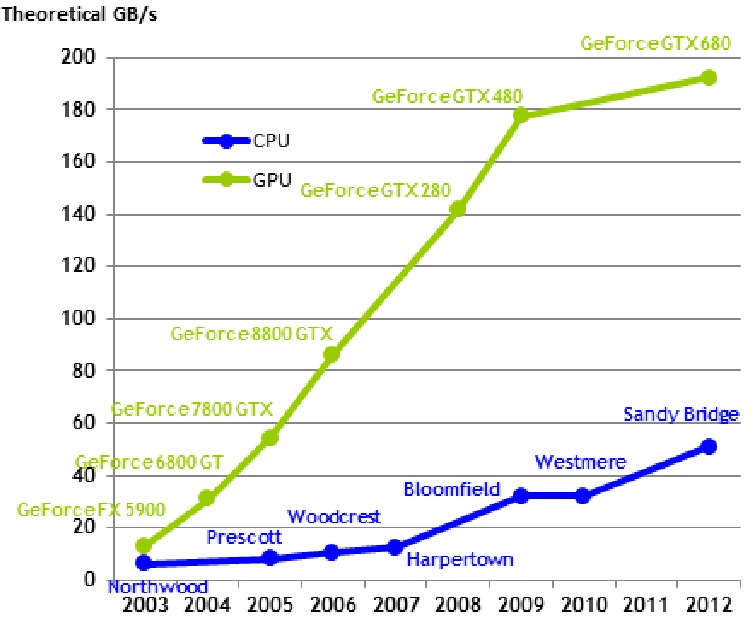
\includegraphics[height=45ex]{img/gpubandwidth.png}
\end  {center}

\end{frame}

\begin{frame}[fragile,t]
\frametitle{GPUs and GFLOPS}

\begin{center}
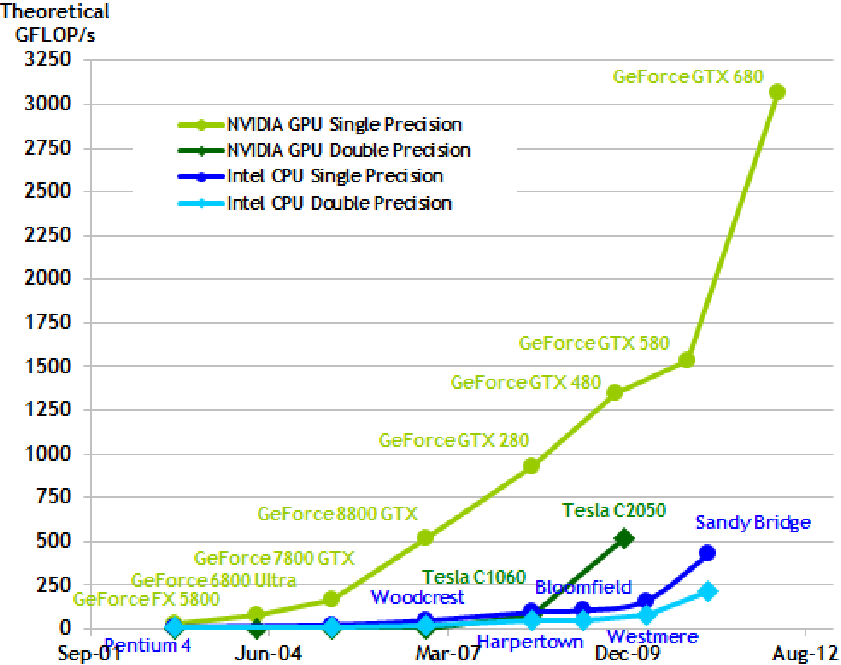
\includegraphics[height=43ex]{img/gpugflops.png}
\end  {center}

\end{frame}


\section{The GPU architecture}

\begin{frame}
	\tableofcontents[currentsection]
\end{frame}

\begin{frame}
  The following slides are taken from the presentation
  \textit{Introduction to GPU Architecture} by Ofer Rosenberg of AMD.
\end{frame}

{
\setbeamercolor{background canvas}{bg=}
\includepdf[pages=4-45]{img/Introduction-to-GPUs.pdf}
}

\section{The OpenCL programming model}

\begin{frame}
	\tableofcontents[currentsection]
\end{frame}


\begin{frame}
  \frametitle{OpenCL for this course}

  \begin{itemize}
  \item OpenCL is a standard C API for programming GPUs and other
    ``accelerators''.
  \item OpenCL is very low-level and very boilerplate-heavy.
  \item Any real application will build domain-specific abstraction
    layers on top.
  \item Since we want to teach you \textit{actual} OpenCL, we can't do
    that, but we will use a small library of abbreviations and
    helpers: \texttt{clutils.h}
  \end{itemize}

  \bigskip

  \hfill
\includegraphics[width=0.25\textwidth]{img/opencl-logo.png}

  \url{https://www.khronos.org/registry/OpenCL/sdk/1.0/docs/man/xhtml/}

\end{frame}

\begin{frame}
  \frametitle{OpenCL is an SIMT model}

  \textit{Single Instruction Multiple Threads} means we provide a
  \textit{sequential function} that is executed in parallel by
  multiple threads (``work items'' in OpenCL).

  \begin{center}
    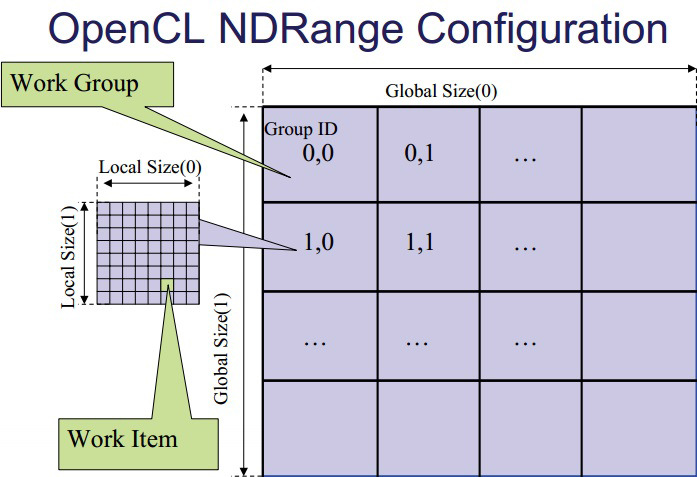
\includegraphics[width=0.75\textwidth]{img/ndrange.png}
  \end{center}

Threads are arranged in \textit{workgroups}, which form an
\textit{NDRange} (often called \textit{grid}).

\end{frame}

\begin{frame}
  \frametitle{OpenCL Platforms and Devices}

  A \textit{platform} is more like a \textit{vendor} (technically, an
  OpenCL backend or driver).  Each platform provides access to zero or
  more \textit{devices}.

  \begin{center}
    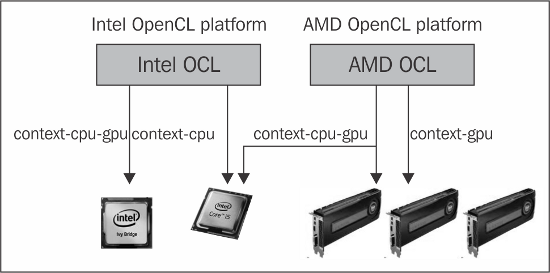
\includegraphics[width=\textwidth]{img/opencl-platforms-devices.png}
  \end{center}

  To use OpenCL, we must pick a \textit{platform}, then one of its
  \textit{devices}, use that to create a \textit{context}, and then a
  \textit{command queue} to which we can finally enqueue device
  operations.
\end{frame}

\begin{frame}[fragile,fragile]
  \frametitle{Listing available devices (Day1/devices.c)}

\begin{lstlisting}[backgroundcolor=\color{lightgray}]
cl_int clGetPlatformIDs
  (cl_uint num_entries,
   cl_platform_id *platforms,
   cl_uint *num_platforms)
\end{lstlisting}

\begin{lstlisting}
cl_uint num_platforms;

// Find the number of platforms.
OPENCL_SUCCEED(
  clGetPlatformIDs(0, NULL, &num_platforms));

printf("Found %d platforms\n",
       (int)num_platforms);
\end{lstlisting}

  The \texttt{OPENCL\_SUCCEED()} macro translates OpenCL error codes
  to strings and aborts the process in case of error.  Proper error
  handling is inherently application-specific and left as a very
  boring exercise.
\end{frame}

\begin{frame}[fragile]
\begin{lstlisting}
// Make room for them.
cl_platform_id *all_platforms =
  calloc(num_platforms, sizeof(cl_platform_id));

// Fetch all the platforms.
OPENCL_SUCCEED(
  clGetPlatformIDs(num_platforms,
                   all_platforms,
                   NULL));

for (unsigned int i = 0; i < num_platforms; i++) {
  ...
}
\end{lstlisting}
\end{frame}

\begin{frame}[fragile,fragile]
\begin{lstlisting}[backgroundcolor=\color{lightgray}]
cl_int clGetPlatformInfo
  (cl_platform_id platform,
   cl_platform_info param_name,
   size_t param_value_size,
   void *param_value,
   size_t *param_value_size_ret)
\end{lstlisting}

\begin{lstlisting}
size_t req_bytes;
char *name;

// How much space do we need for the platform name?
OPENCL_SUCCEED(
  clGetPlatformInfo(all_platforms[i],
                    CL_PLATFORM_NAME,
                    0, NULL,
                    &req_bytes));
\end{lstlisting}
\end{frame}

\begin{frame}[fragile]
\begin{lstlisting}
// Allocate space for the name and fetch it.
name = malloc(req_bytes);
OPENCL_SUCCEED(
  clGetPlatformInfo(all_platforms[i],
                    CL_PLATFORM_NAME,
                    req_bytes, name,
                    NULL));

printf("Platform %d: %s\n", i, name);

free(name);
\end{lstlisting}
\end{frame}

\begin{frame}[fragile]
\begin{lstlisting}
// Now let us print the names of all the devices,
// first we count how many of them exist.
cl_uint num_devices;
OPENCL_SUCCEED(
  clGetDeviceIDs(all_platforms[i],
                 CL_DEVICE_TYPE_ALL,
                 0, NULL,
                 &num_devices));

// Then we make room for them.
cl_device_id *platform_devices =
  calloc(num_devices, sizeof(cl_device_id));

// Then we fetch them.
OPENCL_SUCCEED(
  clGetDeviceIDs(all_platforms[i],
                 CL_DEVICE_TYPE_ALL,
                 num_devices, platform_devices,
                 NULL));
\end{lstlisting}
\end{frame}

\begin{frame}[fragile]
\begin{lstlisting}
for (unsigned int j = 0; j < num_devices; j++) {
  // How much space do we need for the device name?
  OPENCL_SUCCEED(
    clGetDeviceInfo(platform_devices[j],
                    CL_DEVICE_NAME,
                    0, NULL, &req_bytes));

  // Allocate space for the name and fetch it.
  name = malloc(req_bytes);
  OPENCL_SUCCEED(
    clGetDeviceInfo(platform_devices[j],
                    CL_DEVICE_NAME,
                    req_bytes, name, NULL));

  printf("\tDevice %d: %s\n", j, name);
  free(name);
}
\end{lstlisting}
\end{frame}

\begin{frame}
  \frametitle{OpenCL in Visual Studio}

  \begin{block}{Warning}
    Neither Cosmin nor I are Windows users and we are entirely
    unexperienced with Visual Studio.
  \end{block}

  \begin{enumerate}
  \item Ensure the AMD OpenCL SDK is installed.
  \end{enumerate}

\end{frame}

\section{Debugging and Profiling OpenCL}

\begin{frame}
	\tableofcontents[currentsection]
\end{frame}

\begin{frame}[fragile,fragile]
  \frametitle{Profiling with Wall Clock Time}

Just like how you profile anything else.

\begin{lstlisting}
// Current wall time in microseconds.
static int64_t get_wall_time(void);
\end{lstlisting}

Use it like this:

\begin{lstlisting}
int64_t before = get_wall_time();

...

clFinish(ctx);

int64_t after = get_wall_time();

printf("Took %d microseconds\n",
       (int)(after-before));
\end{lstlisting}

The \lstinline{clFinish()} call is crucial as otherwise the device may
still be working (remember that most enqueuings are
\textit{asynchronous}).

\end{frame}

\begin{frame}[fragile]
  \frametitle{Profiling with Events}

  An event is an object that communicates the status of an OpenCL
  command.  Whenever we enqueue something in a command queue, we can
  get an event object back.

\begin{lstlisting}[backgroundcolor=\color{lightgray}]
 cl_int clEnqueueNDRangeKernel
   (cl_command_queue command_queue,
    cl_kernel kernel,
    cl_uint work_dim,
    const size_t *global_work_offset,
    const size_t *global_work_size,
    const size_t *local_work_size,
    cl_uint num_events_in_wait_list,
    const cl_event *event_wait_list,
    @cl_event *event@)
\end{lstlisting}

\end{frame}

\begin{frame}[fragile]
  \frametitle{Retrieving Information from Events}

\begin{lstlisting}[backgroundcolor=\color{lightgray}]
cl_int clGetEventInfo
  (cl_event event,
   cl_event_info param_name,
   size_t param_value_size,
   void *param_value,
   size_t *param_value_size_ret)
\end{lstlisting}

\begin{lstlisting}
 cl_int clGetEventProfilingInfo
   (cl_event event,
    cl_profiling_info param_name,
    size_t param_value_size,
    void *param_value,
    size_t *param_value_size_ret)
\end{lstlisting}

  The latter only works if \lstinline{CL_QUEUE_PROFILING_ENABLE} was
  passed to \lstinline{clCreateCommandQueue()}.
\end{frame}

\begin{frame}[fragile]
  \frametitle{Values for \texttt{cl\_profiling\_info}}

  \begin{description}
  \item[\texttt{CL\_PROFILING\_COMMAND\_QUEUED}]\hfill\\ When the
    command was queued.
  \item[\texttt{CL\_PROFILING\_COMMAND\_SUBMIT}]\hfill\\ When the
    command was sent to the device.
  \item[\texttt{CL\_PROFILING\_COMMAND\_START}]\hfill\\ When the
    command started executing.
  \item[\texttt{CL\_PROFILING\_COMMAND\_END}]\hfill\\ When the
    command finished executing.
  \end{description}

  \begin{itemize}
  \item All produce a value of type \lstinline{cl_ulong}.
  \item \lstinline{clGetEventProfilingInfo()} returns
    \lstinline{CL_PROFILING_INFO_NOT_AVAILABLE} if the information is
    not available (yet)
  \end{itemize}
\end{frame}

\begin{frame}[fragile]
  \frametitle{Example of Profiling with Events}

\begin{lstlisting}
cl_event write_e;
clEnqueueWriteBuffer(queue, to, CL_FALSE,
                     0, n,
                     from,
                     0, NULL, &write_e));

...

cl_ulong start, end;

clGetEventProfilingInfo
  (write_e, CL_PROFILING_COMMAND_START,
   sizeof(start), &start, NULL);
clGetEventProfilingInfo
  (write_e, CL_PROFILING_COMMAND_START,
   sizeof(end), &end, NULL);
\end{lstlisting}

\end{frame}

\begin{frame}
  \frametitle{Event Profiling versus Wall Clock Profiling}

  \begin{itemize}
  \item Event profiling is \textbf{much more fine-grained} and lets us
    see the per-operation runtime.
  \item Measuring per-operation with wall clock would require us to
    \texttt{clFinish()} after every operation, which is very slow
    because it prevents pipelining.
  \item Wall clock profiling tells us about \textbf{overall
      application performance}.  We generally cannot just sum the
    runtimes for each event, since the commands may overlap in time,
    and the events do not count host-based overheads.
  \item \textbf{Ideally, use both.}
  \end{itemize}

  However, neither of these approaches will tell us \textit{why}
  something is slow...
\end{frame}

\section{Programming Exercises}

\begin{frame}
	\tableofcontents[currentsection]
\end{frame}


\end{document}

%%% Local Variables:
%%% mode: latex
%%% TeX-master: t
%%% End:
